\newpage 

\section{Compiler Optimizations for Thread-Level Speculation \cite{zhai2002compiler} }
 While using  multithreaded hardware to improve the throughput of a
workload is straightforward, using it to improve the performance
of a single application requires parallelization. The ideal solution
would be to convert sequential programs into parallel programs automatically, but unfortunately this is difficult (if not impossible) for
many general-purpose programs due to their use of pointers, complex data and control struetures, and run-time inputs.


Thread-Level Speculation (TLS) is a potential solution to this problem since it allows the
compiler to create parallel threads without having to prove that
they are independent. The underlying hardware ensures that interthread dependences through memory are satisfied, and re-executes
any thread for which they are not.

The key to extracting parallelism from these programs and hence
improving performance is in the efficiency of speculative execution. While recent research has investigated hardware optimization
for TLS, there has been relatively little work
on compiler optimization in this area. One potential opportunity
for optimization focuses on data dependences between speculative
threads that occur frequently: if the compiler is able to identify the
source and the destination of a frequent inter-thread data dependence,
then it is beneficial to insert synchronization and forward
that value explicitly to avoid failed speculation. Figure l(a) shows
an example loop that the compiler has speculatively parallelized by
partitioning the loop into speculative threads (aka epochs). Since
the variable A is read and written in every iteration,
the compiler decides to synchronize and forward A by inserting a wa i t operation
before the first use of A, and a signal operation after the last definition of A--we describe, implement, and evaluate this algorithm
in Section 3. The synchronization results in the partially-parallel
execution shown in Figure l(a), where each epoch stalls until the
value of A is produced by the previous epoch. The flow of the value
of A between epochs serializes the parallel execution, and so we refer to it as a critical forwarding path.
The overall performance of speculation is limited by the size of
this critical forwarding path.

\begin{figure}[H]
	\centering
	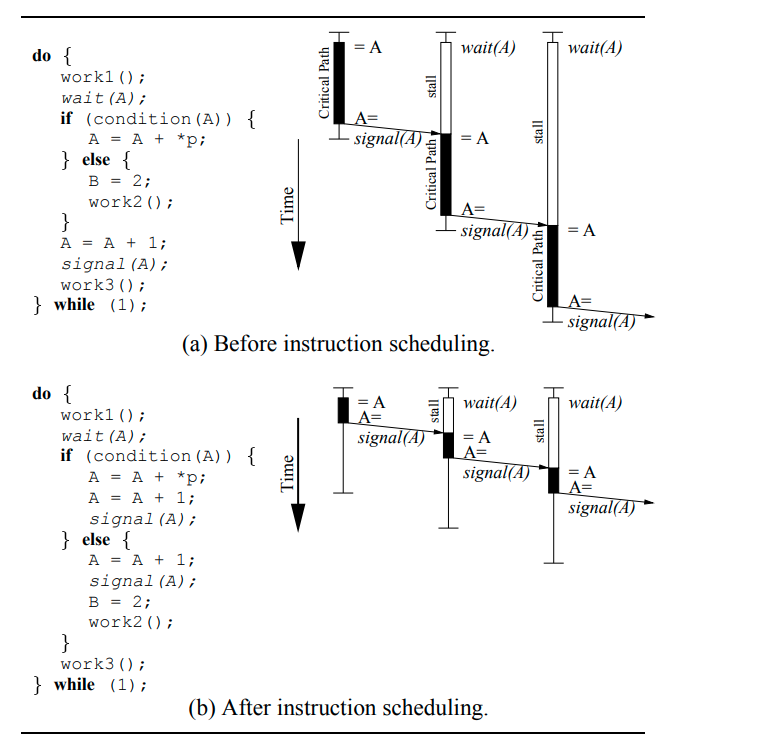
\includegraphics[width=0.5\textwidth]{p207.png}
	\caption{ Impact of scheduling on the critical forwarding path.}
	\label{fig:p207}
\end{figure}

Compiler can improve the performance of speculatively parallelized code by
using scheduling techniques to move the signal operations (and the code that these operations depend upon)
upwards through the control flow graph to reduce the length of the
critical forwarding path and expose more parallelism.

\subsubsection{Scheduling Instructions Speculatively}







